\chapter{Results} \label{chap:results}

This chapter presents the results of the developer study, the academic literature
analysis, the open-source repository analysis and the thematic classification,
validation and consolidation of the logging guideline catalogue. The results are presented according
to the four research questions and are discussed in more detail in
Chapter~\ref{chap:conclusion}.

\section{Developer Study Results}
This section addresses RQ1: \textit{What logging practices and challenges do
software developers encounter in software development and maintenance?}
The results cover developers' experiences with logging during implementation,
log analysis and fault localisation. Quantitative survey responses are presented
together with the practices and challenges reported in the free-text responses.

\subsection{Survey Response Overview}

The survey dataset contained 26 recorded responses, including both complete and
partial questionnaires. Ten participants reached the final section of the
questionnaire. For the analyses presented in this chapter, missing responses were
excluded question by question rather than interpreted as negative answers.
Therefore, the number of responses included in the analysis differs by question
and is specified where necessary.
\\
The three parts of the developer study examined logging implementation, log analysis
and fault localisation. Eight respondents provided usable answers for the logging
implementation section, seven respondents answered the log-analysis section and six
respondents answered the fault-localisation section.
\\
Selected results are presented in the following subsections. Additional survey
figures, detailed response distributions and the paraphrased open-ended responses
are provided in Appendix~\ref{appendix:logging-implementation},
Appendix~\ref{appendix:log-analysis} and
Appendix~\ref{appendix:fault-localisation}.


\subsection{Logging Implementation Practices}

Eight respondents provided usable answers for the logging implementation section.
The reported share of overall development time spent implementing logging ranged
from 3\% to 90\%, with a median of 10\%
(Figure~\ref{fig:results-implementation-time}).

\begin{figure}[H]
    \centering
    \begin{minipage}{0.92\textwidth}
        \centering
        \textbf{\small
        What percentage of your overall development time do you spend
        implementing logging?}
    \end{minipage}
    \resizebox{0.75\textwidth}{!}{%
        \vspace{0.7em}
        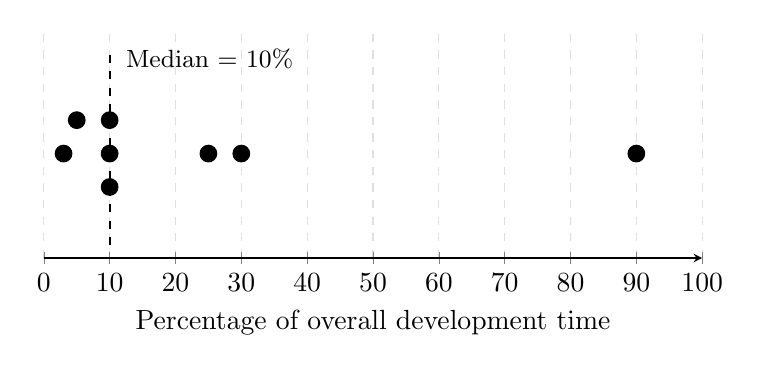
\begin{tikzpicture}
            \begin{axis}[
                width=0.82\textwidth,
                height=4.5cm,
                xmin=0,
                xmax=100,
                ymin=0.75,
                ymax=1.30,
                xlabel={Percentage of overall development time},
                xtick={0,10,20,30,40,50,60,70,80,90,100},
                ytick=\empty,
                axis y line=none,
                axis x line=bottom,
                grid=major,
                grid style={dashed,gray!25},
                clip=false
            ]
            \addplot[
                only marks,
                mark=*,
                mark size=3pt
            ] coordinates {
                (3,1.00)
                (5,1.08)
                (10,0.92)
                (10,1.00)
                (10,1.08)
                (25,1.00)
                (30,1.00)
                (90,1.00)
            };
            % Median = 10%
            \draw[dashed,thick]
                (axis cs:10,0.78) --
                (axis cs:10,1.25);
            \node[
                anchor=south west,
                font=\small
            ] at (axis cs:11,1.18)
            {Median = 10\%};
            \end{axis}
        \end{tikzpicture}
    }
    \caption{Percentage of overall development time spent implementing
    logging among respondents who implement logging.}
    \label{fig:results-implementation-time}
\end{figure}

The implementation questions examined what developers log, which methods and tools
they use, how they determine the criticality of information and which logging
decisions they perceive as difficult. Because multiple selections were possible for
several questions, the percentages in the following figures do not sum to 100\%.
\\
Regarding the type of information recorded, event reporting was the most frequently
represented category, selected by 75\% of respondents (6/8). State-dump information
was reported by 62.5\% (5/8), while execution-tracing information was reported by
50\% (4/8), as shown in Figure~\ref{fig:results-what-to-log}.

\begin{figure}[H]
    \centering
    \begin{minipage}{0.92\textwidth}
        \centering
        \textbf{\small
        What kind of data do you log?}
    \end{minipage}
    \vspace{0.7em}
    \resizebox{0.85\textwidth}{!}{%
        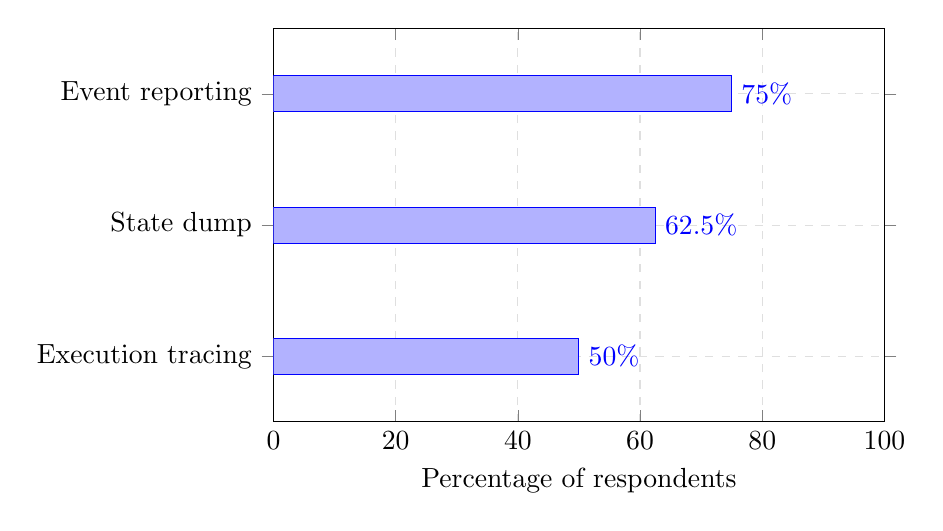
\begin{tikzpicture}
            \begin{axis}[
                xbar,
                width=0.64\textwidth,
                height=5cm,
                scale only axis,
                xmin=0,
                xmax=100,
                xtick={0,20,40,60,80,100},
                xlabel={Percentage of respondents},
                symbolic y coords={
                    {Execution tracing},
                    {State dump},
                    {Event reporting}
                },
                ytick=data,
                nodes near coords,
                nodes near coords={
                    \pgfmathprintnumber{\pgfplotspointmeta}\%
                },
                point meta=x,
                bar width=13pt,
                enlarge y limits=0.25,
                grid=major,
                grid style={dashed,gray!25}
            ]
            \addplot coordinates {
                (50,{Execution tracing})
                (62.5,{State dump})
                (75,{Event reporting})
            };
            \end{axis}
        \end{tikzpicture}
    }
    \caption{Types of information logged according to the
    literature-derived \textit{What to log} codebook.
    Multiple categories could be assigned to one response.}
    \label{fig:results-what-to-log}
\end{figure}

Print statements were the most frequently reported logging method, used by 75\% of
respondents (6/8), followed by off-the-shelf logging frameworks at 62.5\% (5/8).
In-house logging tools, external logging services and self-developed logging
solutions were each reported by 37.5\% (3/8)
(Figure~\ref{fig:results-logging-methods}).

\begin{figure}[H]
    \centering
    \begin{minipage}{0.92\textwidth}
        \centering
        \textbf{\small
        What methods or tools do you use for logging?}
    \end{minipage}
    \vspace{0.7em}
    \resizebox{0.85\textwidth}{!}{%
        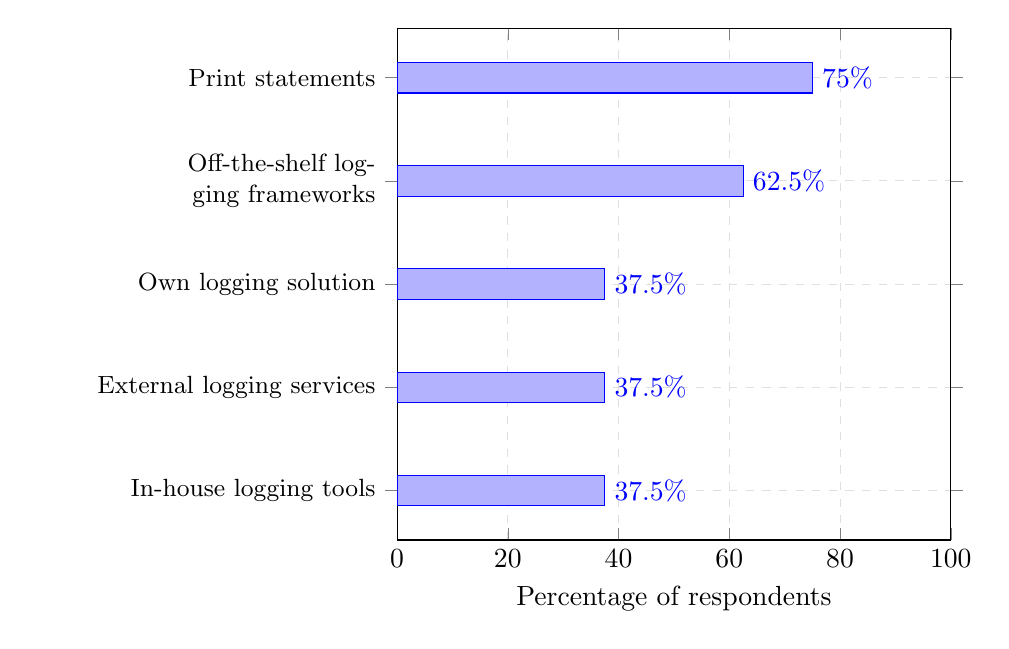
\begin{tikzpicture}
            \begin{axis}[
                xbar,
                width=0.58\textwidth,
                height=6.5cm,
                scale only axis,
                xmin=0,
                xmax=100,
                xtick={0,20,40,60,80,100},
                xlabel={Percentage of respondents},
                symbolic y coords={
                    {In-house logging tools},
                    {External logging services},
                    {Own logging solution},
                    {Off-the-shelf logging frameworks},
                    {Print statements}
                },
                ytick=data,
                yticklabel style={
                    text width=4.3cm,
                    align=right,
                    font=\small
                },
                nodes near coords,
                nodes near coords={
                    \pgfmathprintnumber{\pgfplotspointmeta}\%
                },
                point meta=x,
                bar width=11pt,
                enlarge y limits=0.12,
                grid=major,
                grid style={dashed,gray!25}
            ]
            \addplot coordinates {
                (37.5,{In-house logging tools})
                (37.5,{External logging services})
                (37.5,{Own logging solution})
                (62.5,{Off-the-shelf logging frameworks})
                (75,{Print statements})
            };
            \end{axis}
        \end{tikzpicture}
    }
    \caption{Methods and tools used for logging.
    Multiple selections were possible.}
    \label{fig:results-logging-methods}
\end{figure}


The most frequently selected criteria for determining the criticality of information
to be logged were potential performance impact and user feedback or incident reports,
both selected by 62.5\% of respondents. The affected system part, the frequency of
similar events, and potential security impact were each selected by 50\%. Compliance
or regulatory requirements were selected by 37.5\%. Historical trends, team-lead or
architect recommendations, current system conditions and predefined guidelines or
standards were each selected by 25\%. In contrast, automated tools or algorithms were
selected by 12.5\% (Figure~\ref{fig:results-criticality-criteria}).

\begin{figure}[H]
    \centering
    \begin{minipage}{0.92\textwidth}
        \centering
        \textbf{\small
        Based on which criteria do you determine how critical
        the information to log is?}
    \end{minipage}
    \vspace{0.7em}
    \resizebox{0.85\textwidth}{!}{%
        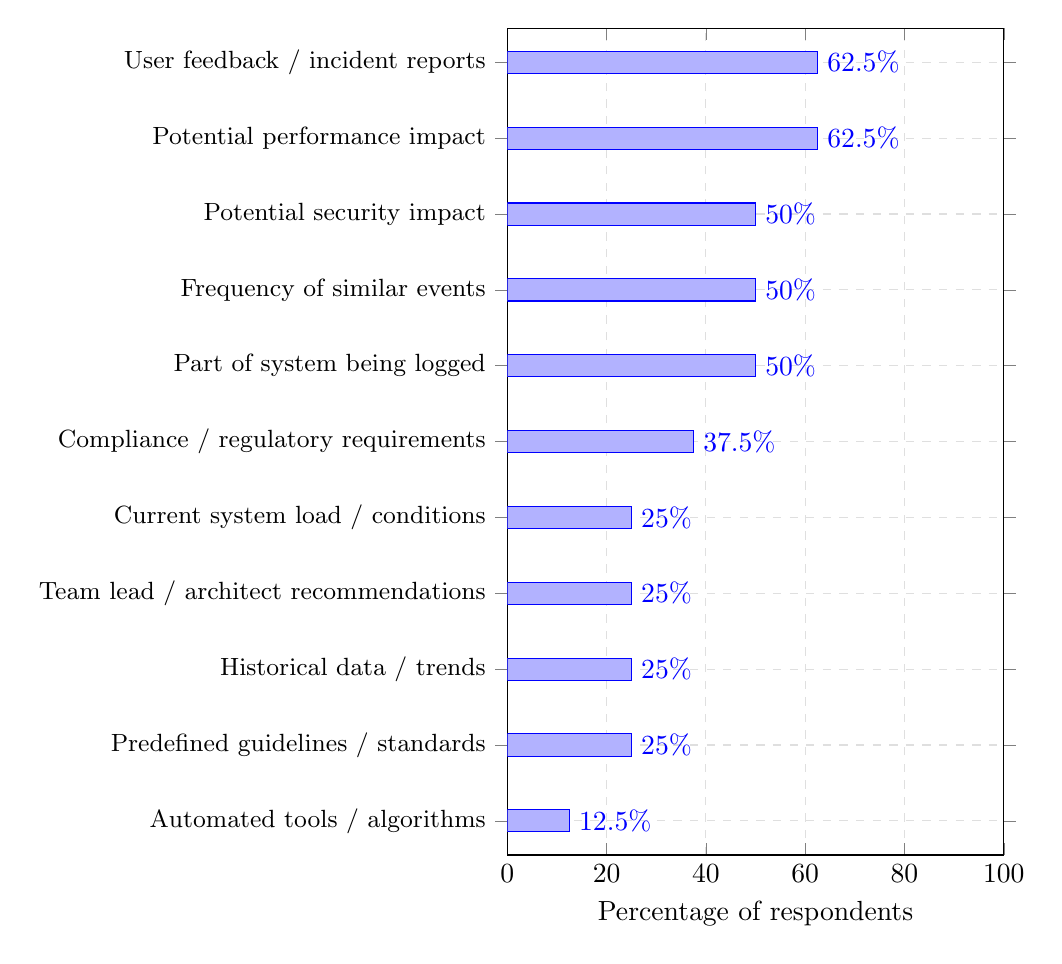
\begin{tikzpicture}
            \begin{axis}[
                xbar,
                width=0.52\textwidth,
                height=10.5cm,
                scale only axis,
                xmin=0,
                xmax=100,
                xtick={0,20,40,60,80,100},
                xlabel={Percentage of respondents},
                symbolic y coords={
                    {Automated tools / algorithms},
                    {Predefined guidelines / standards},
                    {Historical data / trends},
                    {Team lead / architect recommendations},
                    {Current system load / conditions},
                    {Compliance / regulatory requirements},
                    {Part of system being logged},
                    {Frequency of similar events},
                    {Potential security impact},
                    {Potential performance impact},
                    {User feedback / incident reports}
                },
                ytick=data,
                yticklabel style={
                    text width=5.7cm,
                    align=right,
                    font=\small
                },
                nodes near coords,
                nodes near coords={
                    \pgfmathprintnumber{\pgfplotspointmeta}\%
                },
                point meta=x,
                bar width=8pt,
                enlarge y limits=0.045,
                grid=major,
                grid style={dashed,gray!25}
            ]
            \addplot coordinates {
                (12.5,{Automated tools / algorithms})
                (25,{Predefined guidelines / standards})
                (25,{Historical data / trends})
                (25,{Team lead / architect recommendations})
                (25,{Current system load / conditions})
                (37.5,{Compliance / regulatory requirements})
                (50,{Part of system being logged})
                (50,{Frequency of similar events})
                (50,{Potential security impact})
                (62.5,{Potential performance impact})
                (62.5,{User feedback / incident reports})
            };
            \end{axis}
        \end{tikzpicture}
    }
    \caption{Criteria used to determine the criticality of information
    to be logged. Multiple selections were possible.}
    \label{fig:results-criticality-criteria}
\end{figure}


The difficulty statements show that deciding \emph{which data to log} was the most
prominent implementation difficulty among the three logging-decision questions.
Half of the respondents agreed that it was difficult to decide which data should be
logged, compared with 12.5\% agreeing that deciding how to log was difficult.
For deciding when to log, 12.5\% strongly agreed that this was difficult, while 50\%
disagreed and 37.5\% were neutral. Similarly, 62.5\% disagreed that deciding how to
log was difficult. Half of the respondents disagreed or strongly disagreed that their
effort for logging data was high. The responses therefore show a greater reported
difficulty around log-content selection than around the timing or technical mechanism
of logging (Figure~\ref{fig:results-logging-difficulties}).

\begin{figure}[H]
    \centering
    \begin{minipage}{0.92\textwidth}
        \centering
        \textbf{\small
        To which extent do you agree or disagree with the following
        statements?}
    \end{minipage}
    \resizebox{0.85\textwidth}{!}{%
        \vspace{0.7em}
        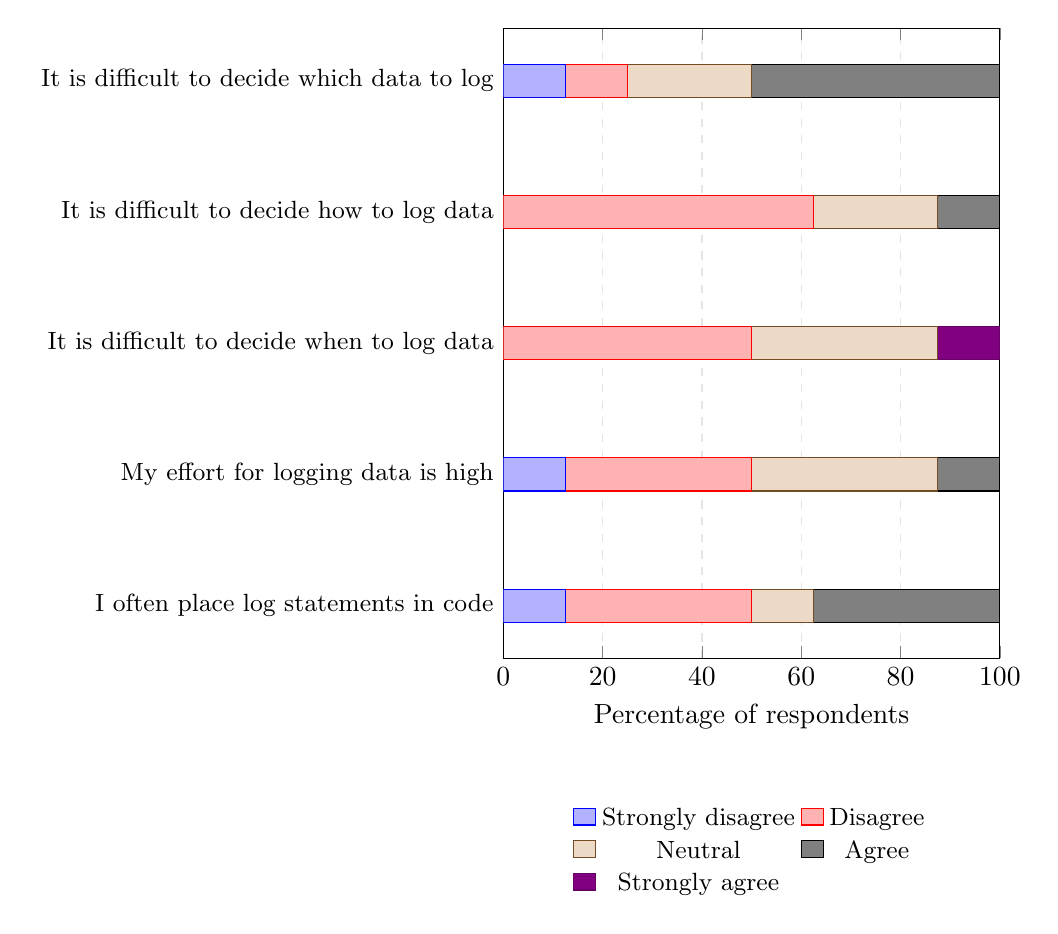
\begin{tikzpicture}
            \begin{axis}[
                xbar stacked,
                width=0.52\textwidth,
                height=8cm,
                scale only axis,
                xmin=0,
                xmax=100,
                xtick={0,20,40,60,80,100},
                xlabel={Percentage of respondents},
                symbolic y coords={
                    {I often place log statements in code},
                    {My effort for logging data is high},
                    {It is difficult to decide when to log data},
                    {It is difficult to decide how to log data},
                    {It is difficult to decide which data to log}
                },
                ytick=data,
                yticklabel style={
                    text width=5.8cm,
                    align=right,
                    font=\small
                },
                bar width=12pt,
                enlarge y limits=0.10,
                legend style={
                    at={(0.5,-0.22)},
                    anchor=north,
                    legend columns=2,
                    font=\small,
                    draw=none
                },
                grid=major,
                grid style={dashed,gray!20}
            ]
            % Strongly disagree
            \addplot coordinates {
                (12.5,{I often place log statements in code})
                (12.5,{My effort for logging data is high})
                (0,{It is difficult to decide when to log data})
                (0,{It is difficult to decide how to log data})
                (12.5,{It is difficult to decide which data to log})
            };
            % Disagree
            \addplot coordinates {
                (37.5,{I often place log statements in code})
                (37.5,{My effort for logging data is high})
                (50,{It is difficult to decide when to log data})
                (62.5,{It is difficult to decide how to log data})
                (12.5,{It is difficult to decide which data to log})
            };
            % Neutral
            \addplot coordinates {
                (12.5,{I often place log statements in code})
                (37.5,{My effort for logging data is high})
                (37.5,{It is difficult to decide when to log data})
                (25,{It is difficult to decide how to log data})
                (25,{It is difficult to decide which data to log})
            };
            % Agree
            \addplot coordinates {
                (37.5,{I often place log statements in code})
                (12.5,{My effort for logging data is high})
                (0,{It is difficult to decide when to log data})
                (12.5,{It is difficult to decide how to log data})
                (50,{It is difficult to decide which data to log})
            };
            % Strongly agree
            \addplot coordinates {
                (0,{I often place log statements in code})
                (0,{My effort for logging data is high})
                (12.5,{It is difficult to decide when to log data})
                (0,{It is difficult to decide how to log data})
                (0,{It is difficult to decide which data to log})
            };
            \legend{
                Strongly disagree,
                Disagree,
                Neutral,
                Agree,
                Strongly agree
            }
            \end{axis}
        \end{tikzpicture}
    }
    \caption{Respondents' perceptions of logging implementation
    practices and difficulties.}
    \label{fig:results-logging-difficulties}
\end{figure}



The open-ended responses provided additional examples of how developers approach
logging implementation in practice. Reported practices included creating clear,
readable and structured log output, placing logs at module or component level to
support execution tracing and using third-party applications for error logging.
Some respondents described considering logging during architecture and design,
using the same logging framework where possible and avoiding both excessive and
insufficient logging.
\\
Other reported practices included recording incoming and outgoing data, writing
meaningful log entries, sampling logs, considering the performance cost of logging
and discussing logging implementation within the development team. The individual
paraphrased responses are provided in
Appendix~\ref{appendix:open-ended-logging-implementation}.

\clearpage
\subsection{Log Analysis Practices}

Seven respondents answered the log-analysis section. Respondents reported
spending between 5\% and 70\% of their overall time analysing logged data, with a
median of 10\% (Figure~\ref{fig:results-log-analysis-time}).

\begin{figure}[H]
    \centering
    \begin{minipage}{0.92\textwidth}
        \centering
        \textbf{\small
        What percentage of your overall time do you spend analysing logged data?}
    \end{minipage}
    \vspace{0.7em}
    \resizebox{0.75\textwidth}{!}{%
        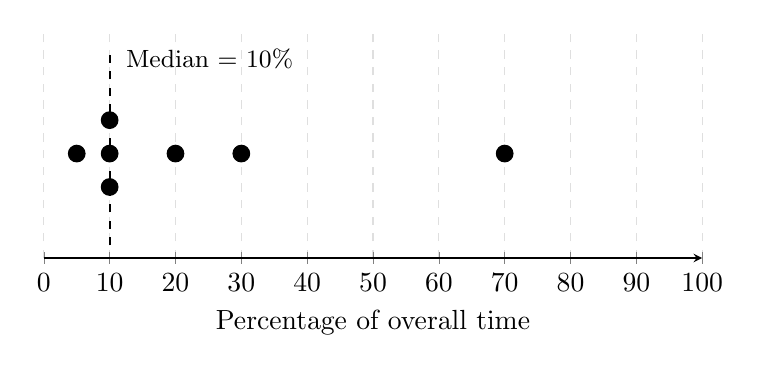
\begin{tikzpicture}
            \begin{axis}[
                width=0.82\textwidth,
                height=4.5cm,
                xmin=0,
                xmax=100,
                ymin=0.75,
                ymax=1.30,
                xlabel={Percentage of overall time},
                xtick={0,10,20,30,40,50,60,70,80,90,100},
                ytick=\empty,
                axis y line=none,
                axis x line=bottom,
                grid=major,
                grid style={dashed,gray!25},
                clip=false
            ]
            \addplot[
                only marks,
                mark=*,
                mark size=3pt
            ] coordinates {
                (5,1.00)
                (10,0.92)
                (10,1.00)
                (10,1.08)
                (20,1.00)
                (30,1.00)
                (70,1.00)
            };
            \draw[dashed,thick]
                (axis cs:10,0.78) --
                (axis cs:10,1.25);
            \node[
                anchor=south west,
                font=\small
            ] at (axis cs:11,1.18)
            {Median = 10\%};
            \end{axis}
        \end{tikzpicture}
    }
    \caption{Percentage of overall time spent analysing logged data among
    respondents who completed the log-analysis section ($n=7$).}
    \label{fig:results-log-analysis-time}
\end{figure}

All seven respondents reported using logged data for debugging or resolving
failures. Identifying failures and locating faults were each reported by 85.7\%
(6/7), customer-reported errors by 57.1\% (4/7), and performance monitoring by
28.6\% (2/7) (Figure~\ref{fig:results-log-analysis-reasons}).

\begin{figure}[H]
    \centering
    \begin{minipage}{0.92\textwidth}
        \centering
        \textbf{\small
        Why do you analyse logged data?}
    \end{minipage}
    \vspace{0.7em}
    \resizebox{0.85\textwidth}{!}{%
        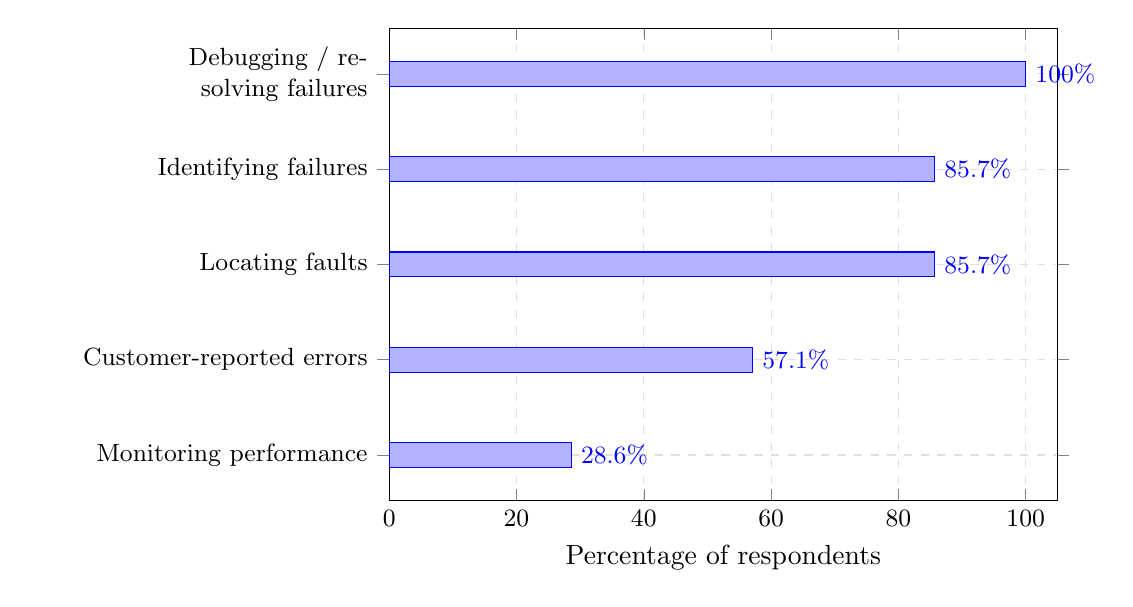
\begin{tikzpicture}
            \begin{axis}[
                xbar,
                width=0.70\textwidth,
                height=6.0cm,
                scale only axis,
                xmin=0,
                xmax=105,
                xtick={0,20,40,60,80,100},
                xlabel={Percentage of respondents},
                symbolic y coords={
                    {Monitoring performance},
                    {Customer-reported errors},
                    {Locating faults},
                    {Identifying failures},
                    {Debugging / resolving failures}
                },
                ytick=data,
                yticklabel style={
                    text width=4.2cm,
                    align=right,
                    font=\small
                },
                tick label style={font=\small},
                nodes near coords={
                    \pgfmathprintnumber[fixed,precision=1]
                    {\pgfplotspointmeta}\%
                },
                every node near coord/.append style={
                    font=\small
                },
                point meta=x,
                bar width=9pt,
                enlarge y limits=0.12,
                grid=major,
                grid style={dashed,gray!25}
            ]
            \addplot coordinates {
                (28.6,{Monitoring performance})
                (57.1,{Customer-reported errors})
                (85.7,{Locating faults})
                (85.7,{Identifying failures})
                (100,{Debugging / resolving failures})
            };
            \end{axis}
        \end{tikzpicture}
    }
    \caption{Reported reasons for analysing logged data
    ($n=7$). Multiple selections were possible.}
    \label{fig:results-log-analysis-reasons}
\end{figure}


A majority of respondents considered structured log messages easier to analyse:
42.9\% agreed, and 14.3\% strongly agreed. The same distribution
was observed for the preference for analysing information logged by oneself.
At the same time, 57.1\% agreed that logs are generally overwhelming. For
failure-related logs, 50\% agreed or strongly agreed that the available information
can be overwhelming, while 33.3\% were neutral
(Figure~\ref{fig:results-log-analysis-perceptions}).

\begin{figure}[H]
    \centering
    \begin{minipage}{0.92\textwidth}
        \centering
        \textbf{\small
        To which extent do you agree or disagree with the following statements?}
    \end{minipage}
    \vspace{0.7em}
    \resizebox{0.85\textwidth}{!}{%
        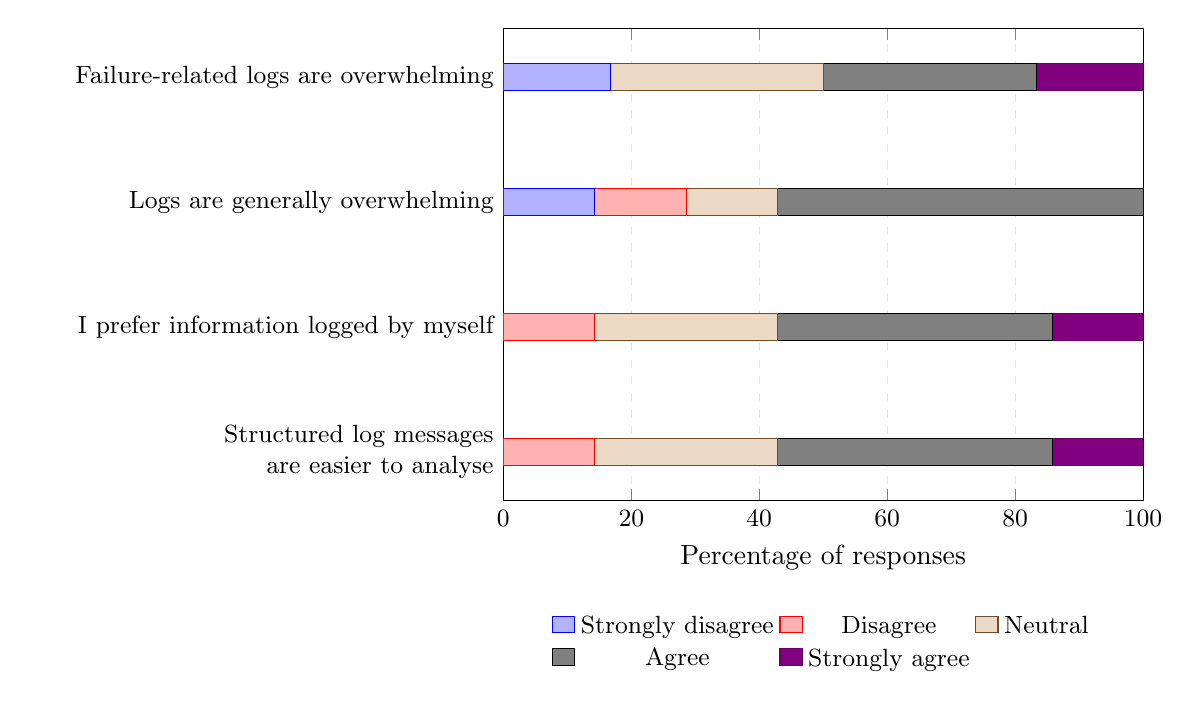
\begin{tikzpicture}
            \begin{axis}[
                xbar stacked,
                width=0.67\textwidth,
                height=6.0cm,
                scale only axis,
                xmin=0,
                xmax=100,
                xtick={0,20,40,60,80,100},
                xlabel={Percentage of responses},
                symbolic y coords={
                    {Structured log messages are easier to analyse},
                    {I prefer information logged by myself},
                    {Logs are generally overwhelming},
                    {Failure-related logs are overwhelming}
                },
                ytick=data,
                yticklabel style={
                    text width=5.8cm,
                    align=right,
                    font=\small
                },
                tick label style={font=\small},
                bar width=10pt,
                enlarge y limits=0.13,
                legend style={
                    at={(0.5,-0.22)},
                    anchor=north,
                    legend columns=3,
                    font=\small,
                    draw=none
                },
                grid=major,
                grid style={dashed,gray!20}
            ]
            % Strongly disagree
            \addplot coordinates {
                (0,{Structured log messages are easier to analyse})
                (0,{I prefer information logged by myself})
                (14.3,{Logs are generally overwhelming})
                (16.7,{Failure-related logs are overwhelming})
            };
            % Disagree
            \addplot coordinates {
                (14.3,{Structured log messages are easier to analyse})
                (14.3,{I prefer information logged by myself})
                (14.3,{Logs are generally overwhelming})
                (0,{Failure-related logs are overwhelming})
            };
            % Neutral
            \addplot coordinates {
                (28.6,{Structured log messages are easier to analyse})
                (28.6,{I prefer information logged by myself})
                (14.3,{Logs are generally overwhelming})
                (33.3,{Failure-related logs are overwhelming})
            };
            % Agree
            \addplot coordinates {
                (42.9,{Structured log messages are easier to analyse})
                (42.9,{I prefer information logged by myself})
                (57.1,{Logs are generally overwhelming})
                (33.3,{Failure-related logs are overwhelming})
            };
            % Strongly agree
            \addplot coordinates {
                (14.3,{Structured log messages are easier to analyse})
                (14.3,{I prefer information logged by myself})
                (0,{Logs are generally overwhelming})
                (16.7,{Failure-related logs are overwhelming})
            };
            \legend{
                Strongly disagree,
                Disagree,
                Neutral,
                Agree,
                Strongly agree
            }
            \end{axis}
        \end{tikzpicture}
    }
    \caption{Respondents' perceptions of log analysis.
    The failure-related-log statement is based on six responses;
    the remaining statements are based on seven responses.}
    \label{fig:results-log-analysis-perceptions}
\end{figure}


Analysis of unfamiliar logs was relatively infrequent. Five of the seven respondents
(71.4\%) selected ``less frequently'', while one respondent reported analysing
unfamiliar logs daily and one weekly. Collaborative log review was also generally
infrequent: 42.9\% selected ``less frequently'', 28.6\% monthly, 14.3\% daily, and
14.3\% never (Figure~\ref{fig:results-log-analysis-frequency}).

\begin{figure}[H]
    \centering
    \begin{minipage}{0.92\textwidth}
        \centering
        \textbf{\small
        How often do you perform the following log analysis activities?}
    \end{minipage}
    \vspace{0.7em}
    \resizebox{0.85\textwidth}{!}{%
        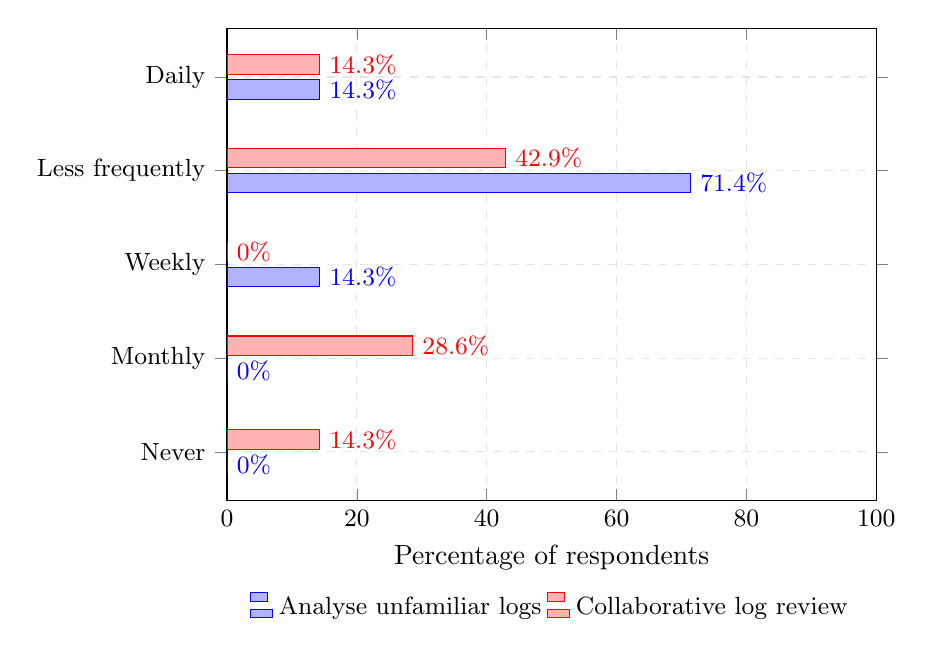
\begin{tikzpicture}
            \begin{axis}[
                xbar,
                width=0.68\textwidth,
                height=6.0cm,
                scale only axis,
                xmin=0,
                xmax=100,
                xtick={0,20,40,60,80,100},
                xlabel={Percentage of respondents},
                symbolic y coords={
                    {Never},
                    {Monthly},
                    {Weekly},
                    {Less frequently},
                    {Daily}
                },
                ytick=data,
                yticklabel style={
                    font=\small
                },
                tick label style={font=\small},
                nodes near coords={
                    \pgfmathprintnumber[fixed,precision=1]
                    {\pgfplotspointmeta}\%
                },
                every node near coord/.append style={
                    font=\small
                },
                point meta=x,
                bar width=7pt,
                enlarge y limits=0.13,
                legend style={
                    at={(0.5,-0.18)},
                    anchor=north,
                    legend columns=2,
                    font=\small,
                    draw=none
                },
                grid=major,
                grid style={dashed,gray!20}
            ]

            % Analysis of unfamiliar logs
            \addplot coordinates {
                (0,{Never})
                (0,{Monthly})
                (14.3,{Weekly})
                (71.4,{Less frequently})
                (14.3,{Daily})
            };

            % Collaborative log review
            \addplot coordinates {
                (14.3,{Never})
                (28.6,{Monthly})
                (0,{Weekly})
                (42.9,{Less frequently})
                (14.3,{Daily})
            };

            \legend{
                Analyse unfamiliar logs,
                Collaborative log review
            }

            \end{axis}
        \end{tikzpicture}
    }
    \caption{Reported frequency of analysing unfamiliar logs and
    reviewing logs collaboratively ($n=7$).}
    \label{fig:results-log-analysis-frequency}
\end{figure}


Semi-structured logs were the most commonly analysed format (5/7 respondents),
followed by structured logs (2/7). No respondent reported unstructured logs as the
primary format analysed.
\\
The open-ended responses provided additional information about how developers perform
log analysis in practice. Respondents described selecting relevant logs based on the
affected component, recent builds or operations, previous experience, log naming
conventions and the reported source of a problem. Several responses described linking
log information back to the corresponding source code to understand the
execution flow or identify the location of an error.
\\
Reported analysis techniques included searching for error strings, timestamps, and
other relevant keywords, locating recent error or warning messages, tracing the
corresponding source code and examining changes in system input, output or state.
Some respondents additionally described consulting documentation, other developers
or AI-supported tools when log information was difficult to interpret.
\\
Reported recommendations included using clear and consistent log structures,
understanding the relevant component and execution flow, using text search to locate
relevant information and formatting logs so that important information can be
identified more easily. The individual paraphrased responses are provided in
Appendix~\ref{appendix:open-ended-log-analysis}.


\subsection{Fault Localization Practices}

The fault-localisation section contained six valid responses. Respondents reported
spending between 3\% and 25\% of their overall time localising faults, with a median
of 12.5\%, as shown in Figure~\ref{fig:results-fault-localization-time}.

\begin{figure}[H]
    \centering
    \textbf{\small
    What percentage of your overall time do you spend localising faults?}

    \vspace{0.5em}
    \resizebox{0.75\textwidth}{!}{%
        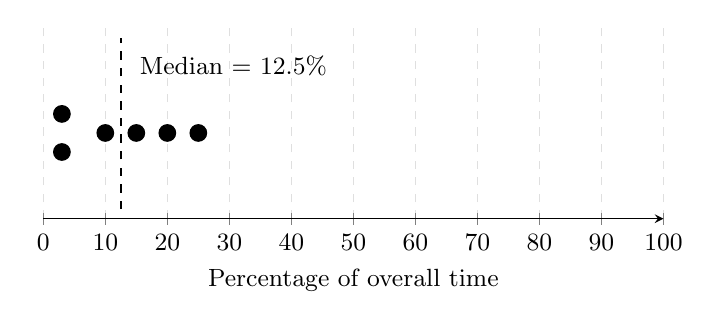
\begin{tikzpicture}
            \begin{axis}[
                width=0.78\textwidth,
                height=4.0cm,
                xmin=0,
                xmax=100,
                ymin=0.82,
                ymax=1.22,
                xtick={0,10,20,30,40,50,60,70,80,90,100},
                xlabel={Percentage of overall time},
                xlabel style={font=\small},
                tick label style={font=\small},
                ytick=\empty,
                axis y line=none,
                axis x line=bottom,
                grid=major,
                grid style={dashed,gray!25},
                clip=false
            ]

            \addplot[
                only marks,
                mark=*,
                mark size=3pt
            ] coordinates {
                (3,0.96)
                (3,1.04)
                (10,1.00)
                (15,1.00)
                (20,1.00)
                (25,1.00)
            };

            \draw[dashed,thick]
                (axis cs:12.5,0.84) --
                (axis cs:12.5,1.20);

            \node[
                anchor=south west,
                font=\small
            ] at (axis cs:14,1.10)
            {Median = 12.5\%};

            \end{axis}
        \end{tikzpicture}
    }
    \caption{Percentage of overall time spent localising faults
    among respondents in the fault-localisation section ($n=6$).}
    \label{fig:results-fault-localization-time}
\end{figure}


The time required to localise a single fault varied between respondents.
Five of the six respondents (83.3\%) reported that fault localisation took
hours on average, while one respondent (16.7\%) reported an average duration
of days. The maximum reported localisation time was generally longer:
66.7\% reported several days, while 16.7\% reported hours and 16.7\%
reported weeks (Figure~\ref{fig:results-fault-localization-duration}).

\begin{figure}[H]
    \centering
    \textbf{\small
    How long does it take to localise the fault of a single failure?}

    \vspace{0.5em}
    \resizebox{0.85\textwidth}{!}{%
        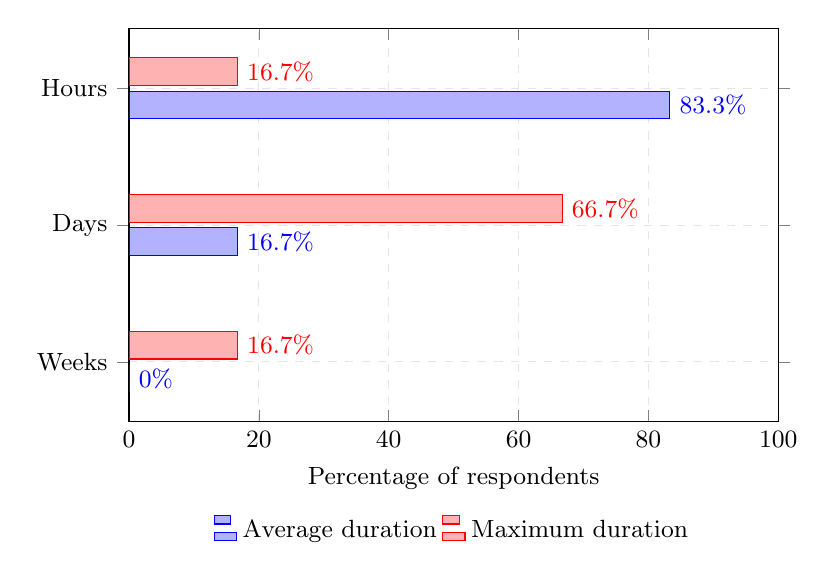
\begin{tikzpicture}
            \begin{axis}[
                xbar,
                width=0.68\textwidth,
                height=5.0cm,
                scale only axis,
                xmin=0,
                xmax=100,
                xtick={0,20,40,60,80,100},
                xlabel={Percentage of respondents},
                xlabel style={font=\small},
                symbolic y coords={
                    {Weeks},
                    {Days},
                    {Hours}
                },
                ytick=data,
                yticklabel style={font=\small},
                tick label style={font=\small},
                bar width=10pt,
                enlarge y limits=0.22,
                nodes near coords={
                    \pgfmathprintnumber[fixed,precision=1]
                    {\pgfplotspointmeta}\%
                },
                every node near coord/.append style={
                    font=\small
                },
                point meta=x,
                legend style={
                    at={(0.5,-0.22)},
                    anchor=north,
                    legend columns=2,
                    font=\small,
                    draw=none
                },
                grid=major,
                grid style={dashed,gray!20}
            ]

            \addplot coordinates {
                (0,{Weeks})
                (16.7,{Days})
                (83.3,{Hours})
            };

            \addplot coordinates {
                (16.7,{Weeks})
                (66.7,{Days})
                (16.7,{Hours})
            };

            \legend{Average duration, Maximum duration}

            \end{axis}
        \end{tikzpicture}
    }
    \caption{Reported average and maximum duration required to localise
    the fault of a single failure ($n=6$).}
    \label{fig:results-fault-localization-duration}
\end{figure}

The knowledge requirements varied by area. Domain or project knowledge received the
highest proportion of ``advanced'' responses at 50\%. Architecture knowledge was
most frequently rated ``moderate'' (66.7\%), while development-process or evolution
history and responsibilities or group organisation were each rated ``moderate'' by
50\%. Knowledge of the language or technology stack was most commonly rated
``limited'' (50\%). Logging knowledge and log-analysis knowledge were also most
frequently rated ``limited'' (50\%), although a third of respondents considered
advanced logging knowledge necessary
(Figure~\ref{fig:results-fault-localization-knowledge}).

\begin{figure}[H]
    \centering
    \textbf{\small
    How much knowledge is required for fault localization?}

    \vspace{0.5em}
    \resizebox{0.85\textwidth}{!}{%
        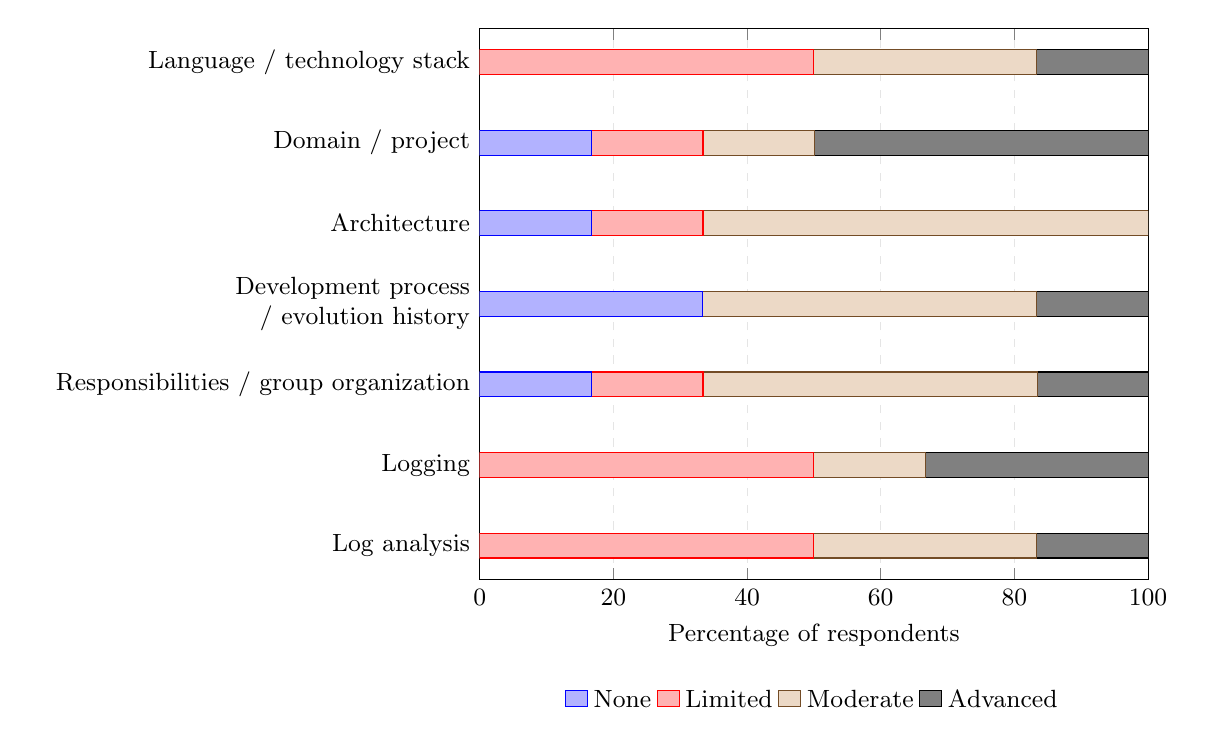
\begin{tikzpicture}
            \begin{axis}[
                xbar stacked,
                width=0.70\textwidth,
                height=7.0cm,
                scale only axis,
                xmin=0,
                xmax=100,
                xtick={0,20,40,60,80,100},
                xlabel={Percentage of respondents},
                xlabel style={font=\small},
                symbolic y coords={
                    {Log analysis},
                    {Logging},
                    {Responsibilities / group organization},
                    {Development process / evolution history},
                    {Architecture},
                    {Domain / project},
                    {Language / technology stack}
                },
                ytick=data,
                yticklabel style={
                    text width=5.5cm,
                    align=right,
                    font=\small
                },
                tick label style={font=\small},
                bar width=9pt,
                enlarge y limits=0.07,
                legend style={
                    at={(0.5,-0.18)},
                    anchor=north,
                    legend columns=4,
                    font=\small,
                    draw=none
                },
                grid=major,
                grid style={dashed,gray!20}
            ]
            % None
            \addplot coordinates {
                (0,{Log analysis})
                (0,{Logging})
                (16.7,{Responsibilities / group organization})
                (33.3,{Development process / evolution history})
                (16.7,{Architecture})
                (16.7,{Domain / project})
                (0,{Language / technology stack})
            };
            % Limited
            \addplot coordinates {
                (50,{Log analysis})
                (50,{Logging})
                (16.7,{Responsibilities / group organization})
                (0,{Development process / evolution history})
                (16.7,{Architecture})
                (16.7,{Domain / project})
                (50,{Language / technology stack})
            };
            % Moderate
            \addplot coordinates {
                (33.3,{Log analysis})
                (16.7,{Logging})
                (50,{Responsibilities / group organization})
                (50,{Development process / evolution history})
                (66.7,{Architecture})
                (16.7,{Domain / project})
                (33.3,{Language / technology stack})
            };
            % Advanced
            \addplot coordinates {
                (16.7,{Log analysis})
                (33.3,{Logging})
                (16.7,{Responsibilities / group organization})
                (16.7,{Development process / evolution history})
                (0,{Architecture})
                (50,{Domain / project})
                (16.7,{Language / technology stack})
            };
            \legend{
                None,
                Limited,
                Moderate,
                Advanced
            }
            \end{axis}
        \end{tikzpicture}
    }
    \caption{Reported level of knowledge required for fault localisation
    across different areas ($n=6$).}
    \label{fig:results-fault-localization-knowledge}
\end{figure}


Cross-component behaviour was a prominent difficulty. All respondents agreed or
strongly agreed that faults involving interactions between system parts are harder to
identify. Furthermore, 83.3\% agreed or strongly agreed that logs from different
system parts are analysed, and 83.3\% agreed that logs are analysed multiple times
during fault localisation. Two thirds of respondents agreed or strongly agreed that
the available logged data is suitable for fault localisation. In contrast, only
33.3\% agreed that logs lack required information, while 50\% disagreed with this
statement. Responses concerning the analysis of non-useful logs were evenly divided:
50\% agreed or strongly agreed and 50\% disagreed or strongly disagreed
(Figure~\ref{fig:results-fault-localization-experiences}).

\begin{figure}[H]
    \centering
    \textbf{\small
    To which extent do you agree or disagree with the following statements?}

    \vspace{0.5em}
    \resizebox{0.85\textwidth}{!}{%
        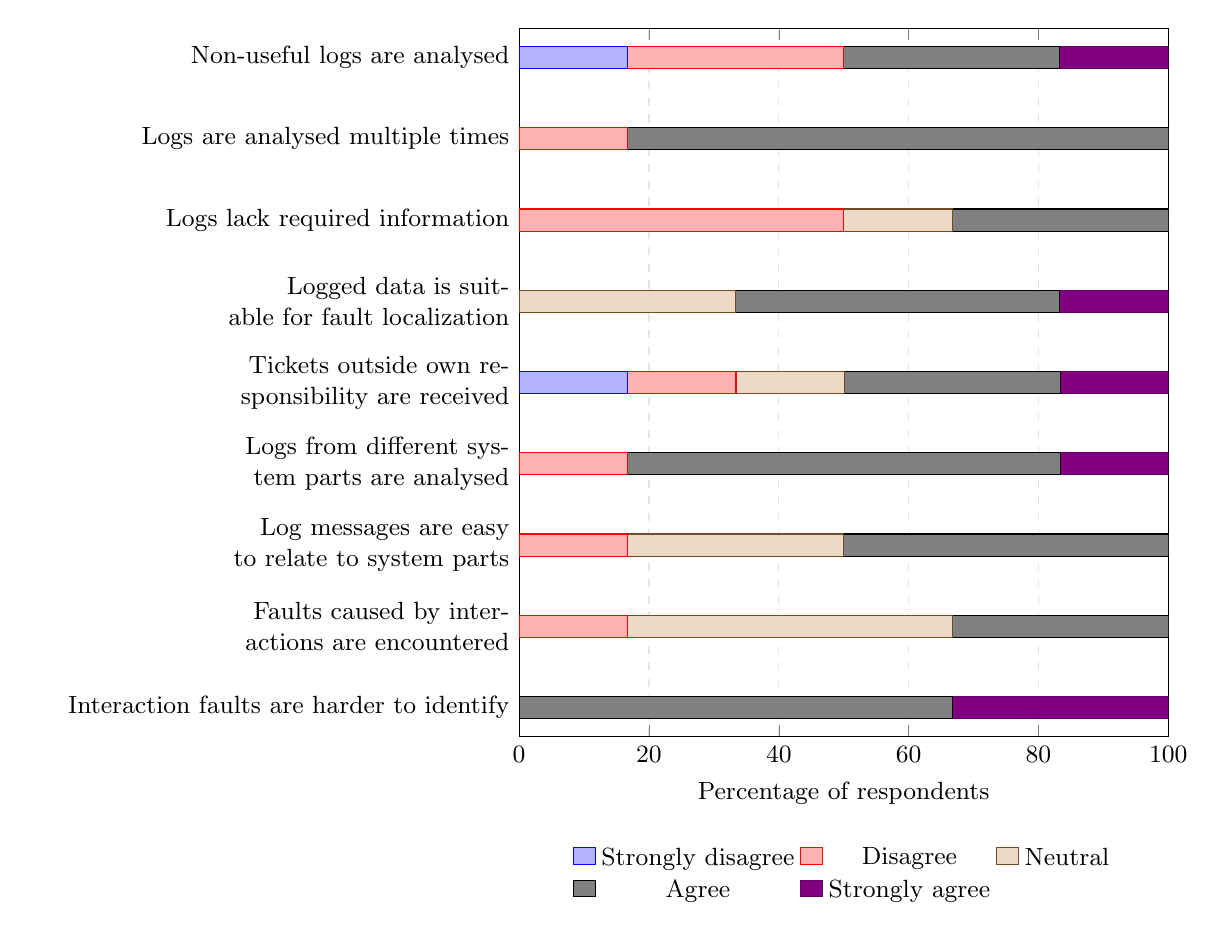
\begin{tikzpicture}
            \begin{axis}[
                xbar stacked,
                width=0.68\textwidth,
                height=9.0cm,
                scale only axis,
                xmin=0,
                xmax=100,
                xtick={0,20,40,60,80,100},
                xlabel={Percentage of respondents},
                xlabel style={font=\small},
                symbolic y coords={
                    {Interaction faults are harder to identify},
                    {Faults caused by interactions are encountered},
                    {Log messages are easy to relate to system parts},
                    {Logs from different system parts are analysed},
                    {Tickets outside own responsibility are received},
                    {Logged data is suitable for fault localization},
                    {Logs lack required information},
                    {Logs are analysed multiple times},
                    {Non-useful logs are analysed}
                },
                ytick=data,
                yticklabel style={
                    text width=6.0cm,
                    align=right,
                    font=\small
                },
                tick label style={font=\small},
                bar width=8pt,
                enlarge y limits=0.045,
                legend style={
                    at={(0.5,-0.14)},
                    anchor=north,
                    legend columns=3,
                    font=\small,
                    draw=none
                },
                grid=major,
                grid style={dashed,gray!20}
            ]
            % Strongly disagree
            \addplot coordinates {
                (0,{Interaction faults are harder to identify})
                (0,{Faults caused by interactions are encountered})
                (0,{Log messages are easy to relate to system parts})
                (0,{Logs from different system parts are analysed})
                (16.7,{Tickets outside own responsibility are received})
                (0,{Logged data is suitable for fault localization})
                (0,{Logs lack required information})
                (0,{Logs are analysed multiple times})
                (16.7,{Non-useful logs are analysed})
            };
            % Disagree
            \addplot coordinates {
                (0,{Interaction faults are harder to identify})
                (16.7,{Faults caused by interactions are encountered})
                (16.7,{Log messages are easy to relate to system parts})
                (16.7,{Logs from different system parts are analysed})
                (16.7,{Tickets outside own responsibility are received})
                (0,{Logged data is suitable for fault localization})
                (50,{Logs lack required information})
                (16.7,{Logs are analysed multiple times})
                (33.3,{Non-useful logs are analysed})
            };
            % Neutral
            \addplot coordinates {
                (0,{Interaction faults are harder to identify})
                (50,{Faults caused by interactions are encountered})
                (33.3,{Log messages are easy to relate to system parts})
                (0,{Logs from different system parts are analysed})
                (16.7,{Tickets outside own responsibility are received})
                (33.3,{Logged data is suitable for fault localization})
                (16.7,{Logs lack required information})
                (0,{Logs are analysed multiple times})
                (0,{Non-useful logs are analysed})
            };
            % Agree
            \addplot coordinates {
                (66.7,{Interaction faults are harder to identify})
                (33.3,{Faults caused by interactions are encountered})
                (50,{Log messages are easy to relate to system parts})
                (66.7,{Logs from different system parts are analysed})
                (33.3,{Tickets outside own responsibility are received})
                (50,{Logged data is suitable for fault localization})
                (33.3,{Logs lack required information})
                (83.3,{Logs are analysed multiple times})
                (33.3,{Non-useful logs are analysed})
            };
            % Strongly agree
            \addplot coordinates {
                (33.3,{Interaction faults are harder to identify})
                (0,{Faults caused by interactions are encountered})
                (0,{Log messages are easy to relate to system parts})
                (16.7,{Logs from different system parts are analysed})
                (16.7,{Tickets outside own responsibility are received})
                (16.7,{Logged data is suitable for fault localization})
                (0,{Logs lack required information})
                (0,{Logs are analysed multiple times})
                (16.7,{Non-useful logs are analysed})
            };
            \legend{
                Strongly disagree,
                Disagree,
                Neutral,
                Agree,
                Strongly agree
            }
            \end{axis}
        \end{tikzpicture}
    }
    \caption{Respondents' reported experiences and challenges during
    fault localisation ($n=6$). Statement labels were shortened for
    readability.}
    \label{fig:results-fault-localization-experiences}
\end{figure}



The open-ended responses provided further examples of how developers perform fault
localisation. Reported practices included tracing an error backwards towards its
underlying cause, identifying the affected functionality through log metadata or
source code and examining the behaviour of the corresponding component.
\\
Respondents also described combining logs with additional information. Examples
included debugger output, variable values, configuration exports, generated files,
database entries and information provided by users or customers. Logs were therefore
not always used as the only source of information during fault localisation.
\\
For failures involving several components, respondents described isolating the
individual functionalities before examining their interaction, contacting developers
responsible for other components and comparing expected system behaviour with the
observed sequence of events. Historical project knowledge was also reported as a
source for understanding interactions between system components. One respondent
described constructing a flowchart of the involved systems and comparing the expected
interaction sequence with the observed behaviour.
\\
The individual paraphrased responses are provided in
Appendix~\ref{appendix:open-ended-fault-localization}.


\subsection{Logging Challenges}

Across the three survey parts, several recurring challenges can be observed in the
structured responses. During implementation, the clearest difficulty concerned the
selection of log content: 50\% of respondents agreed that deciding which data to log
is difficult, whereas fewer respondents reported comparable difficulty in deciding
when or how to log.
\\
During log analysis, the volume and interpretability of available information emerged
as relevant concerns. Although a majority considered structured logs easier to
analyse, 57.1\% agreed that logs are generally overwhelming. Respondents also
encountered unfamiliar logs and collaborative analysis, although these activities
were generally reported less frequently than routine analysis of familiar logs.
\\
During fault localisation, the strongest difficulty concerned failures caused by
interactions across system components. All six respondents considered such faults
harder to identify. The repeated analysis of logs and the need to inspect logs from
different system parts further indicate that fault localisation frequently requires
context beyond a single log statement or component.

\subsection{Answer to RQ1}

RQ1 investigated the logging practices and challenges encountered by software
developers during implementation, log analysis and fault localisation.
\\
For logging implementation, developers reported recording events, system state, and
execution information using mechanisms ranging from print statements to established
logging frameworks and project-specific solutions. The open-ended responses further
described practices such as creating structured and readable logs, considering
logging during architecture and design, using consistent logging frameworks,
recording relevant input and output data and considering logging performance costs.
The most frequently reported implementation difficulty was deciding which information
should be logged.
\\
For log analysis, logs were primarily used for debugging, failure identification and
fault localisation. Reported practices included selecting logs based on the affected
component or previous experience, searching for errors and timestamps, relating log
entries to source code and execution flow and examining changes in system state or
data. Structured logs were generally perceived as easier to analyse, while respondents
also reported that log information can become overwhelming.
\\
For fault localisation, respondents described tracing failures towards their
underlying cause, connecting log entries with affected system components and combining
logs with additional technical and contextual information. Fault localisation also
involved collaboration with developers responsible for other components when several
parts of a system interacted. Failures involving such interactions were consistently
reported as more difficult to identify.
\\
Overall, the survey shows that logging practice extends beyond the creation of log
statements. Developers use logging throughout implementation, analysis and fault
localisation and combine log information with source code, system knowledge,
additional runtime information and collaboration with other developers. At the same
time, the responses show difficulties concerning the selection of useful log content,
the interpretability and volume of log information and the localisation of faults
across interacting system components.

\section{Logging Guidelines from Academic Literature}
\label{sec:results-literature}
This section addresses RQ2: \textit{What logging guidelines are documented in
academic literature?}
The results summarise the selected academic literature, the identified logging
recommendations across the four logging dimensions and the coverage of the
retained actionable recommendations in the final consolidated open-source
catalogue.

\subsection{Literature Search Results}

The literature collection resulted in 31 academic publications relevant to software
logging. In addition, seven logging tools or utilities identified during the
literature analysis were recorded separately as supporting information. These tool
entries were not counted as independent academic publications.
\\
The literature search combined publications identified directly through the defined
Google Scholar search terms with earlier publications identified through backward
snowballing. The resulting literature set therefore contained both recent studies
and earlier work addressing logging practices, logging decisions, logging
instrumentation and the subsequent use of generated log data.
\\
The selected publications contained different forms of evidence. Some publications
provided explicit or clearly identifiable logging recommendations. In contrast, others
primarily reported empirical observations, conceptual classifications, logging
tools, automated instrumentation approaches, evaluation results or techniques for
processing and analysing logs. Consequently, inclusion in the literature set did
not automatically mean that a publication contributed an actionable recommendation
to the later guideline-level coverage comparison.
\\
For example, \textit{Improving Software Diagnosability via Log Enhancement} was
retained because it contributes relevant research on logging and software
diagnosability. However, the extracted material primarily described the
LogEnhancer approach and its method for improving log information rather than
providing a sufficiently explicit standalone logging recommendation. It was
therefore retained as supporting academic evidence but was not treated as an
independent recommendation target. The same distinction was applied to other
publications whose relevant contribution was primarily empirical, conceptual,
tool-oriented, descriptive or evaluation-based.
\\
A publication was treated as a source of actionable logging guidance only when an
identifiable recommendation prescribed, recommended or clearly demonstrated an
action concerning the creation, configuration or implementation of logging. A
single publication could therefore contribute no actionable recommendation, one
recommendation or several conceptually distinct recommendation targets.
\\
This distinction between the complete literature set and the actionable academic
recommendation set was maintained throughout the subsequent analysis. The complete
set of 31 publications provides the academic context for RQ2, while only the
identified actionable recommendations are used for the later guideline-level
comparison with the consolidated open-source catalogue.


\subsection{Selected Literature}

The selected publications addressed different aspects of software logging. Four
publications were particularly important for the deductive classification used later
in the open-source analysis because they provided the initial structure for the four
high-level logging dimensions.

\begin{table}[H]
    \centering

    \begin{tabularx}{\textwidth}{p{3.0cm} X X}
        \toprule
        \textbf{Dimension} &
        \textbf{Academic basis} &
        \textbf{Literature-derived themes} \\
        \midrule

        What to log &
        \textit{Industry Practices and Event Logging: Assessment of a Critical
        Software Development Process}~
        \cite{peccia2015industrypracticesandeventlogging} &
        State dump, Execution tracing, Event reporting \\

        Where to log &
        \textit{Where Do Developers Log? An Empirical Study on Logging Practices
        in Industry}~
        \cite{fu2014wheredodeveloperslog} &
        Assertion-check, Return-value-check, Exception, Logic-branch,
        Observing-point logging \\

        How to log &
        \textit{A Survey of Software Log Instrumentation}~
        \cite{chen2021asurveyofsoftwareloginstrumentation} &
        Logging approach, Logging utility integration, Logging code composition \\

        Log verbosity &
        Gholamian and Ward~
        \cite{gholamian2021whatdistributedsystemssay} &
        FATAL, ERROR, WARN, INFO, DEBUG, TRACE \\

        \bottomrule
    \end{tabularx}

    \caption{Academic sources used to ground the initial deductive classification.}
    \label{tab:literature-codebook-sources}
\end{table}

These publications provided the deductive starting point for the thematic
classification. The literature-derived themes were not treated as a complete
classification of all logging guidance. Instead, they provided an initial structure
that was later applied to the open-source guideline corpus and extended inductively
where the deductive themes did not sufficiently represent recurring concepts.


\subsection{Extracted Logging Guidelines}

The actionable recommendations identified in the academic literature addressed all
four major logging decisions considered in this thesis: \textit{what to log},
\textit{where to log}, \textit{how to log}, and
\textit{log levels and verbosity}.
\\
Recommendations concerning \textit{what to log} included recording system state,
dynamic values, events, failures, errors and contextual information.
\\
Recommendations concerning \textit{where to log} addressed locations such as
assertion checks, exception handlers, return-value checks, logic branches, observing points and
method or function boundaries.
\\
Within \textit{how to log}, the literature contained guidance concerning structured
and consistent log representations, logging approaches, the integration of logging
utilities, and composing log messages.
\\
The \textit{log levels and verbosity} dimension contained recommendations concerning
the selection and use of severity levels such as FATAL, ERROR, WARN, INFO, DEBUG
and TRACE, as well as the balance between logging detail, usefulness, and operational
cost.
\\
Not every publication contributed a standalone actionable recommendation. Some
publications instead provided empirical findings, classifications, tool descriptions,
evaluation results or broader observations concerning logging. These publications
were retained in the academic literature set but were not forced into the coverage
analysis.
\\
The literature review identified a set of academic logging recommendations that was
kept separate from publications whose contributions were primarily empirical,
conceptual, descriptive or tool-oriented. Depending on its content, a publication
could contribute none, one or several distinct recommendation targets. These targets
were subsequently used as the academic reference set for comparison with the
consolidated open-source catalogue.


\subsection{Coverage in the Open-Source Catalogue}
\label{sec:results-cross-source}

The retained actionable academic recommendations were subsequently compared with
the final consolidated open-source catalogue to assess the extent to which the
recommendations identified in academic literature were represented in the collected
practical guidance.
\\
The comparison was performed at the level of individual actionable recommendations
rather than at publication level. A publication could therefore contribute several
distinct recommendation targets, while publications retained primarily as
empirical, conceptual, descriptive or tool-oriented evidence did not contribute an
independent coverage target.
\\
A recommendation was classified as \textit{fully covered} when one or more
canonical guidelines expressed the same underlying recommendation while preserving
its relevant meaning, scope and conditions. A recommendation was classified as
\textit{partially covered} when the principal logging concern was represented in
the catalogue but one or more relevant aspects, conditions or sub-recommendations
were not represented sufficiently. A recommendation was classified as
\textit{not identified} when no canonical guideline sufficiently represented the
underlying recommendation.
\\
The comparison showed that a substantial part of the actionable academic guidance
was also represented in the collected open-source guidance. Several
recommendations were only partially represented, however, because individual
aspects of the academic guidance were not identified completely in the final
catalogue.
\\
For example, the literature-derived recommendation concerning logging at different
program locations was largely represented through guidelines addressing
return-value checks, exception handling, logic branches and observing points.
However, no open-source guideline in the collected corpus was assigned to
\textit{Assertion-check logging}. Other partial cases concerned recommendations
whose main logging concern was represented in the catalogue but whose complete
combination of conditions or sub-recommendations was not identified.
\\
The comparison therefore indicates substantial overlap between actionable
recommendations documented in academic literature and logging guidance identified
in the collected open-source sources, while also revealing specific aspects of
academic guidance that were only partially represented.


\subsection{Answer to RQ2}

RQ2 investigated which logging guidelines are documented in academic literature.
The literature collection contained 31 academic publications, together with seven
logging tools or utilities recorded separately as supporting information.
\\
The literature contained both actionable logging recommendations and publications
whose contributions were primarily empirical, conceptual, descriptive,
tool-oriented or evaluation-based. Publications without a sufficiently identifiable
actionable logging recommendation were retained as supporting academic evidence but
were not treated as independent recommendation targets.
\\
The actionable recommendations addressed all four logging dimensions considered in
this thesis: \textit{what to log}, \textit{where to log}, \textit{how to log}, and
\textit{log levels and verbosity}. Recommendations included guidance concerning the
information that should be recorded, suitable locations for logging, the
construction and integration of logging mechanisms, and the selection of
appropriate log levels and verbosity.
\\
The academic literature also provided classifications that formed the deductive
starting point for the later thematic analysis of the open-source guideline corpus.
These classifications included State dump, Execution tracing and Event reporting
for \textit{what to log}, five program-location themes for \textit{where to log},
three themes concerning logging implementation for \textit{how to log}, and the
six conventional severity levels from FATAL to TRACE.
\\
Comparison with the consolidated open-source catalogue showed substantial semantic
overlap between the actionable academic recommendations and the practical guidance
identified in open-source sources. Some recommendations were only partially
represented because individual aspects or conditions of the academic guidance were
not identified completely in the collected open-source corpus. In particular,
\textit{Assertion-check logging} remained part of the literature-derived codebook
but was not observed in the collected open-source guidance.

\section{Logging Guidelines from Open-Source Repositories}
\label{sec:results-open-source}
This section addresses RQ3: \textit{What logging guidelines are documented in
open-source repositories?}
The results present the GitHub search and collection results, the characteristics
of the collected sources, the extracted logging guidelines and the construction,
validation and refinement of the final consolidated guideline catalogue.

\subsection{Repository Collection Results}

The GitHub collection was performed using ten search queries defined in the
methodology. The individual query-result files contained 966 search-result rows in
total. Because the same repository or file could be returned by more than one query,
the combined results contained 939 unique file URLs belonging to 895 unique
repositories.
\\
Table~\ref{tab:github-query-results} shows the number of results obtained for each
query.

\begin{table}[H]
    \centering
    \small

    \begin{tabularx}{\textwidth}{l X r}
        \toprule
        \textbf{Query} & \textbf{Search focus} & \textbf{Results} \\
        \midrule
        Query 1 & General logging guidelines, standards, conventions, and policies & 87 \\
        Query 2 & What to log, log levels, structured logging, and sensitive information & 102 \\
        Query 3 & Logging in relation to observability, tracing, telemetry, and engineering practices & 86 \\
        Query 4 & Structured logging, correlation IDs, and trace IDs & 102 \\
        Query 5 & Sensitive data, PII, GDPR, and credentials in logs & 109 \\
        Query 6 & Log levels and severity conventions & 103 \\
        Query 7 & Logging guidance with additional Java and Go focus & 94 \\
        Query 8 & Logging and observability guidance in Markdown documentation & 104 \\
        Query 9 & Observability, telemetry, diagnostics, tracing, and logging practices & 96 \\
        Query 10 & Logging smells, bad practices, and anti-patterns & 83 \\
        \midrule
        \textbf{Total} & & \textbf{966} \\
        \bottomrule
    \end{tabularx}

    \caption{Focus and number of results obtained for the ten GitHub search queries.}
    \label{tab:github-query-results}
\end{table}

The query results formed the initial candidate set for the open-source collection.
Repeated results across queries were removed, and sources that were no longer
available or had been removed were excluded during collection. File-level duplicate
checking was additionally supported by cosine-similarity analysis. Highly similar
files were reviewed to identify duplicate content, while files that remained
meaningfully different were retained. This similarity analysis was used only for
source-file cleaning and was separate from the later semantic consolidation of
individual logging guidelines.
\\
Following the cleaning process, manual relevance review, and the extended source
collection, 229 source files were retained for content extraction. The files
represented 11 file types, with Markdown files forming the majority of the corpus.

\begin{table}[H]
    \centering

    \begin{tabular}{lr}
        \toprule
        \textbf{File type} & \textbf{Files} \\
        \midrule
        \texttt{.md} & 188 \\
        \texttt{.go} & 22 \\
        \texttt{.txt} & 9 \\
        \texttt{.adoc} & 2 \\
        \texttt{.rst} & 2 \\
        \texttt{.yaml} & 1 \\
        \texttt{.mdx} & 1 \\
        \texttt{.pod} & 1 \\
        \texttt{.toml} & 1 \\
        \texttt{.py} & 1 \\
        \texttt{.ts} & 1 \\
        \midrule
        \textbf{Total} & \textbf{229} \\
        \bottomrule
    \end{tabular}

    \caption{File types in the collected logging corpus before content extraction.}
    \label{tab:oss-file-types}
\end{table}

After extraction and contextual processing, 203 source files contributed at least
one extracted row to the structured dataset. Of these, 202 sources contributed at
least one valid logging guideline. The structured dataset contained 2.347 source
rows, consisting of 2.289 valid source-level guideline occurrences and 58 rows
classified as \texttt{NO\_GUIDELINE}.
\\
Among the valid guideline occurrences, 1.885 (82.4\%) originated from repository
sources and 404 (17.6\%) from external or third-party logging sources included in
the catalogue. At source level, 185 repository sources and 17 external or third-party
sources contributed at least one valid guideline.

\subsection{Repository Characteristics}

The collected sources represented a broad range of project contexts, programming
languages and application fields. Metadata were retained for project type,
programming language, application field, repository activity and source provenance.
\\
The metadata labels were kept in their descriptive form rather than being assigned
to a small set of predefined categories. Across the 203 sources contributing extracted content,
the structured corpus contained 200 distinct project-type descriptions, 187 distinct
language or technology descriptions and 200 distinct application-field
descriptions.
\\
For the 185 GitHub repository sources that contributed at least one valid guideline,
repository size and activity were additionally summarised using stars, commits, and
the number of developers or contributors. Because these distributions were not
symmetrically distributed, both mean and median values are reported together with
the observed minimum and maximum.

\begin{table}[H]
    \centering

    \begin{tabular}{lrrrrr}
        \toprule
        \textbf{Repository metric} &
        \textbf{N} &
        \textbf{Mean} &
        \textbf{Median} &
        \textbf{Min.} &
        \textbf{Max.} \\
        \midrule
        Stars & 185 & 188.4 & 2 & 0 & 10.644 \\
        Commits & 185 & 991.3 & 88 & 1 & 52.217 \\
        Developers / contributors & 185 & 12.2 & 2 & 1 & 390 \\
        \bottomrule
    \end{tabular}

    \caption{Descriptive characteristics of the GitHub repositories contributing
    valid logging guidelines.}
    \label{tab:repository-metadata-summary}
\end{table}

The large differences between the mean and median values show that the repository
characteristics were unevenly distributed. The median repository had two stars, 88
commits and two developers or contributors, whereas the observed maxima reached
10.644 stars, 52.217 commits and 390 developers or contributors. The collected
guidance therefore originated from both comparatively small projects and
substantially larger open-source projects. These characteristics are treated as
contextual information about the sources rather than as indicators of guideline
quality.
\\
Repository creation and update dates were also retained as descriptive indicators
of project age and activity. The contributing repositories included projects
created between 2014 and 2026. The available update metadata also showed a large
number of repositories with recent activity, particularly in 2025 and 2026.


\subsubsection{Project Types}

The project types ranged from reusable logging libraries and application frameworks
to educational repositories, cloud-platform guidance, database automation,
command-line tools, workflow engines, desktop utilities and domain-specific
applications. The diversity of project descriptions shows that the collected
logging guidance was not restricted to a single software architecture or
application type.


\subsubsection{Programming Languages}

The language metadata included language-specific repositories as well as
multi-language guideline documents. Frequently represented technologies included
Python, JavaScript/TypeScript, Node.js, Go, Java/Kotlin, Rust and
framework-specific logging stacks. Because several guidance documents addressed
multiple languages, the language information was retained as descriptive metadata
rather than reducing every source to one programming language.


\subsubsection{Application Fields}

The application-field metadata similarly represented heterogeneous contexts,
including cloud and platform engineering, security, education, developer tooling,
workflow orchestration, data platforms, database administration, desktop and
systems software and domain-specific applications.
\\
These metadata were retained in the catalogue to preserve the project context of
individual recommendations and to allow guidelines to be examined according to
their source environment.


\subsection{Extracted Logging Guidelines}

The extraction process produced 2.347 structured source rows. The source
content and its contextual information were retained during the subsequent
normalisation process.
\\
For each extracted item, the source content and its Content Tag were analysed
together to formulate a clear, concise and self-contained logging guideline.
Where the extracted material did not support a meaningful logging recommendation,
the row was classified as \texttt{NO\_GUIDELINE} rather than being forced into the
catalogue.
\\
This resulted in 2.289 valid source-level guideline occurrences and 58
\texttt{NO\_GUIDELINE} rows. The valid occurrences formed the source-level
guideline corpus used for the subsequent thematic classification and consolidation.
\\
In addition, 440 source rows contained code, configuration, input, usage or
program-output material that was identified as relevant example information.
These examples were retained separately as Example Reasons and linked to the
corresponding guideline where applicable.
\\
After thematic classification, semantically equivalent guidelines were consolidated
while preserving differences in recommended action, conditions, scope and
restrictions. Guidelines with uncertain equivalence were retained separately.
\\
Semantic consolidation reduced the 2.289 source-level guideline occurrences to
2.127 canonical guidelines, corresponding to a reduction of approximately 7.1\%.
Most canonical guidelines (2.034) were unique or deliberately retained separately.
Fifty-four consolidation groups resulted from normalised-identical guideline wording,
while 39 groups represented conservative semantic matches. In total, 93 canonical
guidelines represented more than one source-level occurrence.

\begin{table}[H]
    \centering

    \begin{tabularx}{\textwidth}{X r}
        \toprule
        \textbf{Metric} & \textbf{Count} \\
        \midrule
        Collected source files & 229 \\
        Source files contributing extracted rows & 203 \\
        Source files contributing valid guidelines & 202 \\
        Structured source rows & 2.347 \\
        Valid source-level guideline occurrences & 2.289 \\
        \texttt{NO\_GUIDELINE} rows & 58 \\
        Example Reason rows & 440 \\
        Canonical guidelines after consolidation & 2.127 \\
        Unique / kept separate canonical guidelines & 2.034 \\
        Normalized-identical consolidation groups & 54 \\
        Conservative semantic-match groups & 39 \\
        Multi-row consolidation groups & 93 \\
        \bottomrule
    \end{tabularx}

    \caption{Open-source guideline collection, extraction, and consolidation
    results.}
    \label{tab:oss-guideline-summary}
\end{table}

\subsection{Validation and Refinement of the Guideline Catalogue}

The initial thematic classification was subsequently validated against the complete
deductive--inductive codebook. Particular attention was given to broad themes that 
contained a comparatively large number of guidelines. The most prominent case 
was \textit{Logging approach}, to which 794 source-level guidelines had initially been assigned.
\\
The guidelines assigned to this theme were re-examined together with their source Content
and compared against all themes in the final codebook. Following this validation, 378 guidelines
remained classified as \textit{Logging approach}, while 416 were reassigned to more specific themes.
Of these reassigned guidelines, 149 remained within the \textit{How to log} dimension but were
represented more specifically by themes such as \textit{Logging utility integration},
\textit{Logging code composition}, \textit{Log lifecycle management}, \textit{Logging verification},
or \textit{Sensitive-data protection}. A further 267 guidelines were reassigned to themes belonging
to another high-level logging dimension where the source Content supported a more appropriate
interpretation.
\\
Subsequent manual validation of the consolidated mapping resulted in four further
assignment changes, leaving 374 source-level occurrences assigned to
\textit{Logging approach} in the final catalogue.
\\
The same classification logic was subsequently applied across the remaining themes to identify
comparable inconsistencies. Theme assignments were corrected where the original Content supported
a more specific existing theme. The deductive or inductive origin of a theme itself was not changed
during this procedure, it was only the assignment of individual guidelines that was reconsidered.
\\
Following thematic validation, the semantic consolidation was also manually inspected.
Consolidated groups containing more than one source occurrence were compared with their
original Content to determine whether all occurrences represented the same underlying recommendation. 
Where different recommendations had been generalised into the same normalised wording, the affected source 
occurrences were separated. If another canonical guideline already represented the recommendation, 
the occurrence was reassigned to that guideline rather than creating a duplicate canonical recommendation. 
A new canonical guideline was retained only where no sufficiently equivalent existing guideline was identified.
\\
For example, one initially consolidated error-related guideline contained source occurrences related to
several distinct concepts, including error logging, stack traces, correlation identifiers, structured 
error representation, and diagnostic configuration. During manual validation, these occurrences were 
redistributed to existing canonical guidelines representing the corresponding recommendations. 
Only a recommendation concerning pointer dereferencing in structured error representations 
remained as a distinct guideline because no sufficiently equivalent canonical guideline was available.
\\
The final catalogue therefore reflects both semantic consolidation and subsequent manual 
validation of the merged groups while preserving the mapping from each source-level 
occurrence to exactly one canonical guideline.

\subsection{Distribution Across Logging Categories}

Following the final thematic validation, the 2.289 valid source-level guideline
occurrences resulted in 2.293 assignments across the four high-level logging
dimensions. The number of assignments is slightly higher than the number of
source-level guideline occurrences because a small number of guidelines genuinely
addressed more than one logging dimension and therefore retained multiple
dimension assignments.
\\
The largest dimension was \textit{How to log}, with 923 source-level assignments
(40.3\%). \textit{What to log} contained 646 assignments (28.2\%),
\textit{Log levels and verbosity} contained 391 assignments (17.1\%), and
\textit{Where to log} contained 333 assignments (14.5\%).
\\
The distribution shows that practical open-source guidance addressed
\textit{How to log} most frequently, although its share was lower after final
validation than in the initial classification. Reassigning guidelines
from broad themes such as \textit{Logging approach} increased the representation
of the other logging dimensions.
\\
The detailed thematic classification within these four dimensions is presented in
Section~\ref{sec:results-themes}.


\subsection{Answer to RQ3}

RQ3 investigated which logging guidelines are documented in open-source software
repositories. The ten GitHub searches produced 966 search-result rows, representing
939 unique file URLs across 895 repositories before the subsequent cleaning and
source-selection stages.
\\
After removing duplicates, reviewing relevance, and expanding the source collection,
229 source files were retained for content extraction. The retained material
included documentation, source code, configuration files and other repository
artefacts containing potentially relevant logging guidance.
\\
The extraction and contextual processing stages produced 2.347 structured source
rows. Of these, 2.289 contained valid source-level logging guideline occurrences,
while 58 rows were classified as \texttt{NO\_GUIDELINE} because no sufficiently
supported logging recommendation could be derived from the corresponding source
content.
\\
The identified guidance covered a broad range of logging decisions and originated
from heterogeneous project types, programming languages and application fields.
The source material also contained practical code, configuration, input, usage and
program-output examples. A total of 440 such source rows were retained as
\textit{Example Reasons} and linked to the corresponding guidelines where
applicable.
\\
Following guideline normalisation and thematic classification, semantically
equivalent recommendations were consolidated while preserving differences in
recommended action, conditions, scope and restrictions. The consolidation was
subsequently manually validated against the source Content. Where a
consolidated group contained different underlying recommendations, the affected
source occurrences were separated and reassigned to an existing canonical guideline
where an appropriate equivalent was already available. A new canonical guideline
was retained only when no existing guideline adequately represented the
recommendation.
\\
After semantic consolidation and subsequent manual validation, 2.289
valid source-level guideline occurrences were represented by 2.127 canonical
guidelines. This corresponds to a reduction of 162 repeated occurrences, or
approximately 7.1\%. Of the final canonical guidelines, 2.034 represented a single
source occurrence, while 93 represented more than one source occurrence.
\\
The source-to-canonical mapping retained all 2.289 valid occurrences, with every
source-level guideline mapped to exactly one canonical guideline. The resulting
catalogue therefore preserves both the original occurrence of logging guidance in
the collected sources and a less repetitive canonical representation of
semantically equivalent recommendations. The detailed thematic structure of these
guidelines is examined separately in RQ4.

\clearpage
\section{Themes in the Logging Guideline Catalogue}
\label{sec:results-themes}
This section addresses RQ4: \textit{What themes can be identified within the
logging guideline catalogue?}
The results present the validated thematic structure of the catalogue across the four
logging dimensions and show how the initial literature-derived themes were
extended by inductive themes identified in the collected guideline corpus.

\subsection{Thematic Catalogue Overview}

RQ4 investigated which themes can be identified within the logging guideline
catalogue. The thematic analysis was based on the 2.289 valid source-level
guideline occurrences identified in the open-source corpus.
\\
The initial classification used 17 deductive themes derived from the academic
literature. Where a guideline could not be adequately represented by an existing
deductive theme, an additional inductive theme was introduced. After reviewing and
consolidating overlapping inductive concepts, the final codebook contained 28
themes: 17 deductive themes and 11 inductive themes.
\\
Before calculating the final theme distribution, the theme assignments were
validated against the complete deductive--inductive codebook and, where necessary,
against the source Content. This validation was particularly relevant for
broad themes containing a comparatively large number of guidelines.
\\
The most prominent case was \textit{Logging approach}, to which 794 source-level
guideline occurrences had initially been assigned. After re-examination of this theme,
378 occurrences initially remained assigned to
\textit{Logging approach}, while 416 were reassigned to more specific themes.
Of these reassigned occurrences, 149 remained within the \textit{How to log}
dimension, whereas 267 were reassigned to themes belonging to another high-level
logging dimension.
\\
Subsequent manual validation of the consolidated mapping resulted in four further
assignment changes, leaving 374 source-level occurrences assigned to
\textit{Logging approach} in the final catalogue.
\\
Comparable classification inconsistencies identified during this validation were
also corrected across the remaining themes. The validation changed the assignment
of individual guidelines where the guideline and its original Content supported a
more appropriate existing theme. It did not change the deductive or inductive origin
of the themes themselves. Consequently, the distributions reported in the following
subsections represent the final validated classification rather than the initial
AI-assisted assignments.
\\
The semantic consolidation of the catalogue was subsequently reviewed against the
source Content. Consolidated groups containing several source occurrences were
checked to determine whether they represented the same underlying recommendation
without losing a distinct action, condition, restriction or scope. Where a
consolidated group contained semantically different recommendations, the affected
occurrences were separated. If an equivalent canonical guideline already existed
elsewhere in the catalogue, the occurrence was reassigned to that guideline instead
of introducing a duplicate recommendation. New canonical guidelines were retained
only where an existing guideline did not adequately represent the corresponding
recommendation.
\\
After final validation, each of the 2.289 valid source-level occurrences remained
mapped to exactly one canonical guideline. The final catalogue contained 2.127
canonical guidelines.
\\
At theme level, a small number of guidelines genuinely addressed more than one
logging dimension or thematic concept. The 2.289 source-level occurrences therefore
resulted in 2.293 final source-level dimension assignments. This distinction is
maintained in the following tables so that multi-dimensional recommendations are
not artificially forced into a single category.

\begin{table}[H]
    \centering

    \begin{tabular}{lrr}
        \toprule
        \textbf{Dimension} &
        \textbf{Source-level assignments} &
        \textbf{Percentage} \\
        \midrule
        What to log & 646 & 28.2\% \\
        Where to log & 333 & 14.5\% \\
        How to log & 923 & 40.3\% \\
        Log levels and verbosity & 391 & 17.1\% \\
        \midrule
        \textbf{Total assignments} & \textbf{2.293} & \textbf{100.0\%} \\
        \bottomrule
    \end{tabular}

    \caption{Distribution of final source-level assignments across the four
    logging dimensions.}
    \label{tab:dimension-distribution}
\end{table}

At the dimension level, \textit{How to log} remained the largest category after final
validation, accounting for 923 source-level assignments. The remaining assignments
were distributed across \textit{What to log}, \textit{Log levels and verbosity},
and \textit{Where to log}. The following subsections present the detailed
distribution of the validated themes within these four dimensions.

\subsection{What to Log}

Four themes were identified within the \textit{What to log} dimension. Three
themes originated from the deductive literature-based codebook, while
\textit{Sensitive-data exclusion} was introduced inductively.

\begin{table}[H]
    \centering

    \begin{tabularx}{\textwidth}{X l rr}
        \toprule
        \textbf{Theme} &
        \textbf{Basis} &
        \textbf{Source-level} &
        \textbf{Consolidated} \\
        \midrule
        State dump & Deductive & 256 & 246 \\
        Execution tracing & Deductive & 24 & 20 \\
        Event reporting & Deductive & 337 & 309 \\
        Sensitive-data exclusion & Inductive & 29 & 29 \\
        \midrule
        \textbf{Total} & & \textbf{646} & \textbf{604} \\
        \bottomrule
    \end{tabularx}

    \caption{Themes within the \textit{What to log} dimension.}
    \label{tab:themes-what-to-log}
\end{table}

\textit{Event reporting} was the largest theme within this dimension, with 337
source-level occurrences and 309 consolidated assignments. These guidelines
concerned the recording of discrete operational, business, security, lifecycle or
user-related events.
\\
\textit{State dump} was the second largest theme and represented recommendations
concerning the recording of program, request, object, variable or system state so
that the state surrounding an event or failure can later be reconstructed.
\\
\textit{Execution tracing} occurred less frequently and concerned calls,
transitions, execution steps or timing information along an execution path.
\\
The inductive theme \textit{Sensitive-data exclusion} represented explicit
recommendations describing information that should not be recorded, including
credentials, secrets, personal information or other sensitive data. This extended
the \textit{What to log} dimension by including explicit restrictions on log
content in addition to recommendations concerning information that should be
recorded.


\subsection{Where to Log}

The final \textit{Where to log} dimension contained ten themes. Five originated
from the deductive literature-based classification and five were introduced
inductively from the open-source guideline corpus.

\begin{table}[H]
    \centering

    \begin{tabularx}{\textwidth}{
        X
        l
        >{\raggedleft\arraybackslash}p{2.4cm}
        >{\raggedleft\arraybackslash}p{2.8cm}
    }
        \toprule

        \textbf{Theme} &
        \textbf{Basis} &
        \textbf{Source Assignment} &
        \textbf{Consolidated Assignment} \\

        \midrule

        Assertion-check logging & Deductive & 0 & 0 \\
        Return-value-check logging & Deductive & 1 & 1 \\
        Exception logging & Deductive & 16 & 15 \\
        Logic-branch logging & Deductive & 12 & 12 \\
        Observing-point logging & Deductive & 6 & 6 \\
        Log destination & Inductive & 150 & 144 \\
        Log storage and retention & Inductive & 16 & 15 \\
        Logger placement and reuse & Inductive & 9 & 10 \\
        Logging configuration location & Inductive & 4 & 4 \\
        Logging scope & Inductive & 119 & 115 \\

        \midrule

        \textbf{Total} & & \textbf{333} & \textbf{322} \\

        \bottomrule

    \end{tabularx}

    \caption{Themes within the \textit{Where to log} dimension.}
    \label{tab:themes-where-to-log}

\end{table}

The largest themes within this dimension were \textit{Logging scope} and
\textit{Log destination}. \textit{Logging scope} describes the component,
subsystem, operation, logger or audit boundary to which logging applies.
\textit{Log destination} describes where generated log records should be sent,
including files, consoles, syslog facilities and other logging sinks.
\\
\textit{Log storage and retention} covered requirements concerning the persistence,
storage, rotation or retention of generated logging information.
\textit{Logger placement and reuse} concerned the placement and reuse of logger
instances, while \textit{Logging configuration location} described where logging
configuration should be defined or maintained.
\\
The literature-derived program-location themes were represented much less
frequently. \textit{Logic-branch logging} contained 12 source-level occurrences,
\textit{Observing-point logging} six, \textit{Exception logging} 16 and
\textit{Return-value-check logging} one.
\\
No source-level guideline was assigned to \textit{Assertion-check logging}. The
theme was nevertheless retained in the final codebook because it formed part of
the literature-derived deductive classification.
\\
The inductive themes therefore extended the meaning of \textit{Where to log}
beyond source-code control-flow locations. Within the collected practical guidance,
``where'' also referred to the scope in which logging applies, the destination of
generated records, and the location at which logging information is stored or
configured.


\subsection{How to Log}

The \textit{How to log} dimension formed the largest part of the final catalogue.
It contained six themes: three deductive and three inductive.

\begin{table}[H]
    \centering

    \begin{tabularx}{\textwidth}{X l rr}
        \toprule
        \textbf{Theme} &
        \textbf{Basis} &
        \textbf{Source-level} &
        \textbf{Consolidated} \\
        \midrule
        Logging approach & Deductive & 374 & 360 \\
        Logging utility integration & Deductive & 217 & 202 \\
        Logging code composition & Deductive & 242 & 218 \\
        Log lifecycle management & Inductive & 53 & 52 \\
        Logging verification & Inductive & 16 & 16 \\
        Sensitive-data protection & Inductive & 21 & 18 \\
        \midrule
        \textbf{Total} & & \textbf{923} & \textbf{866} \\
        \bottomrule
    \end{tabularx}

    \caption{Themes within the \textit{How to log} dimension.}
    \label{tab:themes-how-to-log}
\end{table}

\textit{Logging approach} was the largest individual theme in the complete
catalogue, with 374 source-level occurrences and 360 consolidated assignments. It
covered recommendations concerning the overall strategy, representation, mode or
general practice used for logging.
\\
The large number of guidelines within this theme does not mean that the guidelines
are semantically equivalent. \textit{Logging approach} functions as a broad
organisational theme, while each guideline retains its specific
recommended action, technical context, conditions and restrictions.
\\
\textit{Logging code composition} contained 242 source-level occurrences and
covered recommendations concerning how log statements, messages, fields, and
structured records should be constructed.
\\
\textit{Logging utility integration} contained 217 occurrences and represented
guidance concerning the integration and configuration of logging frameworks,
handlers, appenders, middleware and related utilities.
\\
Three additional themes emerged inductively. \textit{Log lifecycle management}
covered the management of logging across its operational lifecycle.
\textit{Logging verification} represented recommendations concerning the
verification or testing of logging behaviour, while
\textit{Sensitive-data protection} covered practices such as masking, filtering,
or redacting sensitive information before writing it to logs.


\subsection{Log Levels and Verbosity}

The final \textit{Log levels and verbosity} dimension contained the six
literature-derived severity levels together with two inductively derived themes.

\begin{table}[H]
    \centering

    \begin{tabularx}{\textwidth}{X l rr}
        \toprule
        \textbf{Theme} &
        \textbf{Basis} &
        \textbf{Source-level} &
        \textbf{Consolidated} \\
        \midrule
        FATAL & Deductive & 3 & 3 \\
        ERROR & Deductive & 19 & 19 \\
        WARN & Deductive & 18 & 15 \\
        INFO & Deductive & 48 & 33 \\
        DEBUG & Deductive & 48 & 39 \\
        TRACE & Deductive & 7 & 7 \\
        Log level selection & Inductive & 242 & 215 \\
        Custom verbosity scale & Inductive & 6 & 6 \\
        \midrule
        \textbf{Total} & & \textbf{391} & \textbf{337} \\
        \bottomrule
    \end{tabularx}

    \caption{Themes within the \textit{Log levels and verbosity} dimension.}
    \label{tab:themes-log-verbosity}
\end{table}

The most frequently represented theme was \textit{Log level selection}, with 242
source-level occurrences and 215 consolidated assignments. These guidelines
concerned the selection, configuration or adjustment of an appropriate logging
level rather than prescribing one individual severity level.
\\
Among the six deductive severity levels, DEBUG and INFO were the most frequently
represented, with 48 and 48 source-level occurrences respectively. FATAL and TRACE
were comparatively uncommon.
\\
The inductive \textit{Custom verbosity scale} theme represented recommendations
associated with project-specific verbosity systems that did not directly follow
the conventional FATAL--TRACE hierarchy.


\subsection{Final Thematic Codebook}

The final codebook contained 28 themes across the four logging dimensions. Seventeen
themes originated from the literature-derived deductive codebook, while 11 themes
were introduced inductively from concepts identified within the collected
open-source guidelines.

\begin{table}[H]
    \centering

    \begin{tabularx}{\textwidth}{p{2.7cm} p{2.0cm} X}
        \toprule

        \textbf{Dimension} &
        \textbf{Basis} &
        \textbf{Themes} \\

        \midrule

        What to log &
        Deductive &
        State dump \newline
        Execution tracing \newline
        Event reporting \\

        What to log &
        Inductive &
        Sensitive-data exclusion \\

        Where to log &
        Deductive &
        Assertion-check logging \newline
        Return-value-check logging \newline
        Exception logging \newline
        Logic-branch logging \newline
        Observing-point logging \\

        Where to log &
        Inductive &
        Logging scope \newline
        Log destination \newline
        Log storage and retention \newline
        Logger placement and reuse \newline
        Logging configuration location \\

        How to log &
        Deductive &
        Logging approach \newline
        Logging utility integration \newline
        Logging code composition \\

        How to log &
        Inductive &
        Log lifecycle management \newline
        Logging verification \newline
        Sensitive-data protection \\

        Log levels and verbosity &
        Deductive &
        FATAL \newline
        ERROR \newline
        WARN \newline
        INFO \newline
        DEBUG \newline
        TRACE \\

        Log levels and verbosity &
        Inductive &
        Log level selection \newline
        Custom verbosity scale \\

        \bottomrule
    \end{tabularx}

    \caption{Final thematic codebook by logging dimension and theme origin.}
    \label{tab:final-codebook-summary}
\end{table}

Of the 28 themes retained in the final codebook, 27 were represented by at least
one source-level guideline. \textit{Assertion-check logging} was the only theme
without an observed source-level occurrence.
\\
The final themes function as organisational and analytical categories rather than
as statements that all guidelines assigned to the same theme are semantically
equivalent. This distinction is particularly important for broad themes such as
\textit{Logging approach}. The individual guideline remains the specific actionable
unit, while the theme provides a higher-level structure for organising and analysing
the catalogue.


\subsection{Answer to RQ4}

RQ4 investigated which themes can be identified within the logging guideline
catalogue. The final thematic codebook contained 28 themes across the four
high-level logging dimensions. Seventeen themes were derived deductively from the
academic literature, while 11 additional themes were identified inductively from
recurring concepts in the collected open-source guideline corpus.
\\
Of the 28 themes, 27 appeared in at least one source-level guideline.
The deductive theme \textit{Assertion-check logging} was retained in the
literature-derived codebook but was not observed in the collected open-source
corpus.
\\
Following final validation, the 2.289 source-level guideline occurrences resulted
in 2.293 source-level dimension assignments because a small number of guidelines
genuinely addressed more than one logging dimension. \textit{How to log} remained
the largest dimension, with 923 assignments (40.3\%), followed by
\textit{What to log} with 646 assignments (28.2\%),
\textit{Log levels and verbosity} with 391 assignments (17.1\%), and
\textit{Where to log} with 333 assignments (14.5\%).
\\
Within the final validated classification, \textit{Logging approach} remained the
largest individual theme, with 374 source-level assignments and 360 canonical
assignments. Its final size was substantially lower than in the initial
classification because guidelines better represented by other
themes were reassigned during manual validation.
\\
The inductive analysis extended the initial literature-derived structure in several
areas. Additional themes captured sensitive-data exclusion and protection, logging
scope and destination, log storage and retention, logger placement and logging
configuration location, log lifecycle management, logging verification, general
log-level selection and custom verbosity systems.
\\
The resulting thematic structure therefore combines established literature-derived
logging concepts with additional concerns identified in practical open-source
guidance. The themes provide a higher-level organisation of the catalogue, while
the individual canonical guidelines retain the specific recommendations, conditions
and contextual distinctions required for practical use.